\section{Data acquisition}
\label{sec:data_acquisition}

Different modalities were captured to create a dataset that reproduces a real-world application of HPE for RGB-D cameras. The different modalities are RGB data, depth data, and joint data. While the Nuitrack SDK offers to capture the data from the RGB-D cameras and the joint data, the recorded files cannot, at the time of writing, be read without using the Nuitrack SDK. Therefore, FESDData, a custom RGB-D+HPE capturing and labelling tool was developed. 

FESDData has two main uses which are interlocked. Firstly, it allows capturing predefined, as well as custom, exercises repeatedly automatically making the capturing experience when capturing many different exercises with multiple repetitions more comfortable. Secondly, it allows reviewing and labelling the captured data with error labels. The lightweight nature of FESDData allows it to seamlessly capture both the RGB-D stream and the skeleton data at the same time while ensuring a stable fast framerate. The dataset that is used by FESDModel was captured at a framerate of 30 frames per second. The interface of FESDData can be seen in figure \ref{fig:fesddata}. On the left side of the image the interface can be seen and on the right, there is an example for data labelling of Exercise E1-02.


\begin{figure}
  \centering
  \begin{subfigure}[b]{0.49\linewidth}
      \centering
      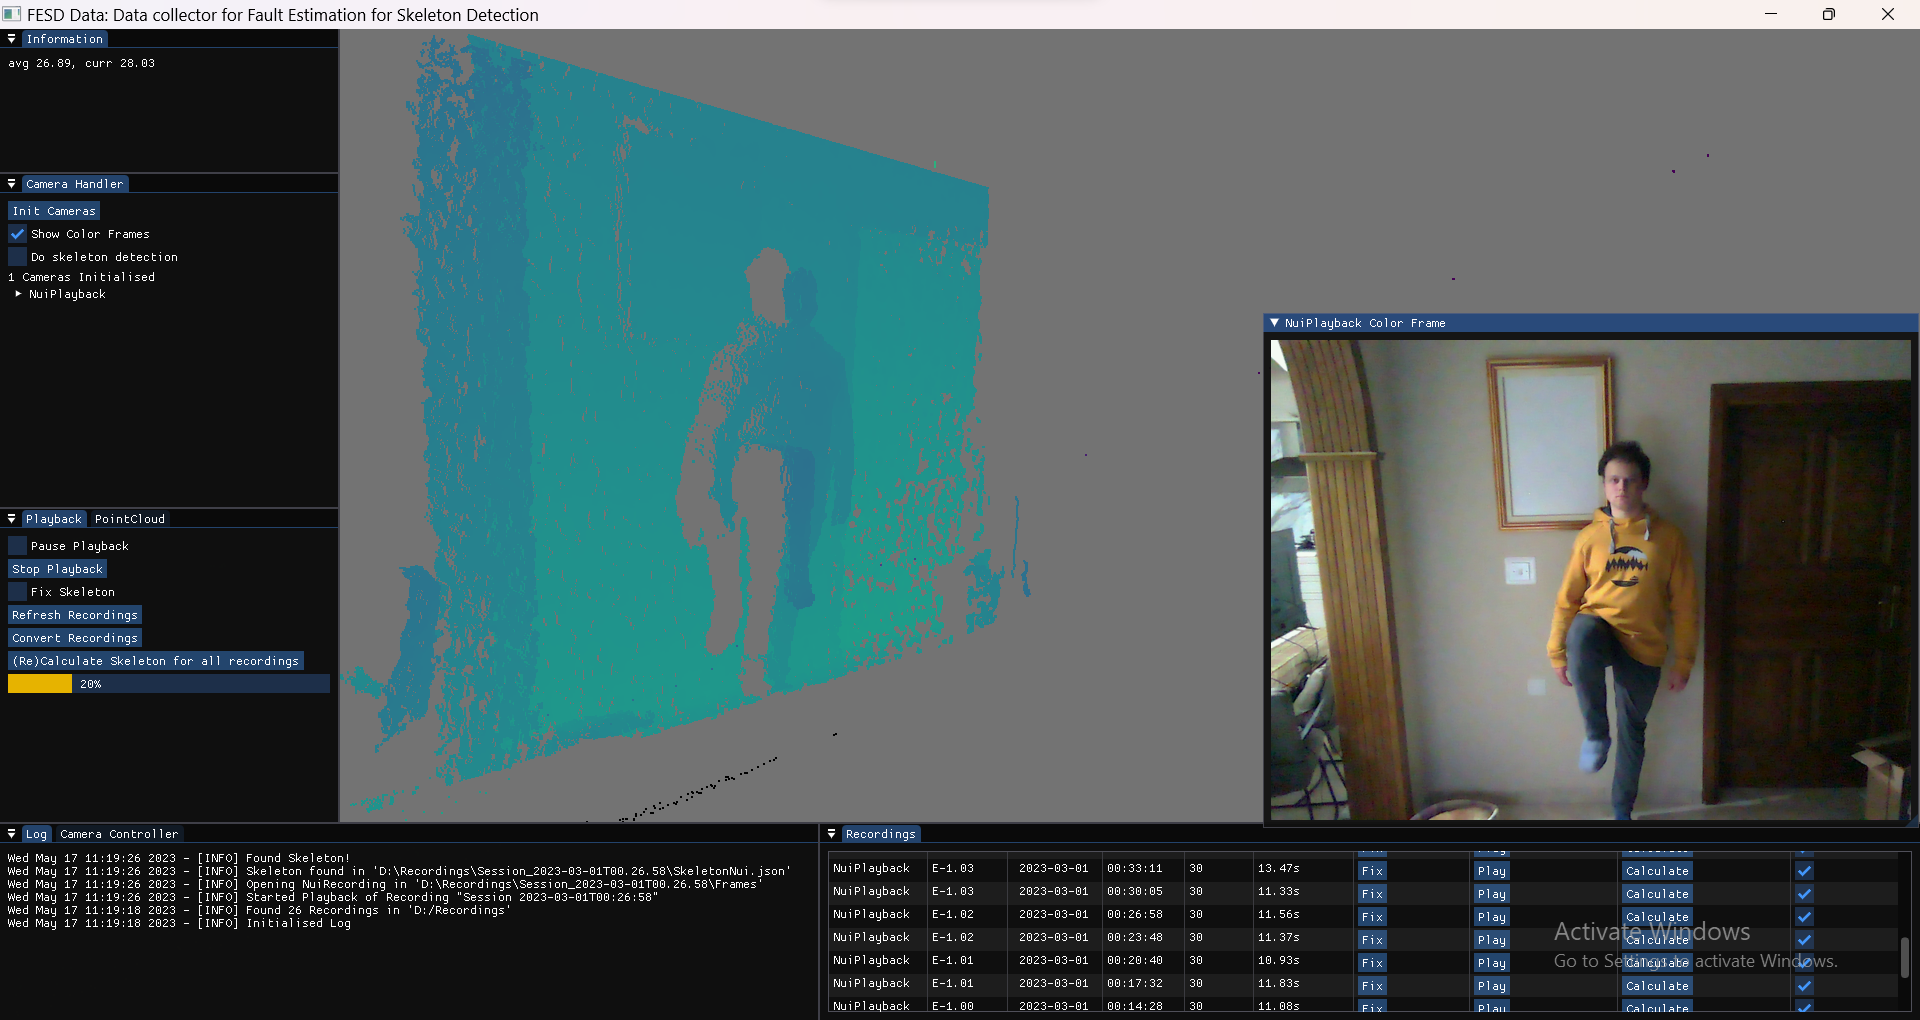
\includegraphics[width=\textwidth]{figures/FESDData/streaming.png}
  \end{subfigure}
  \hfill
  \begin{subfigure}[b]{0.49\linewidth}
      \centering
      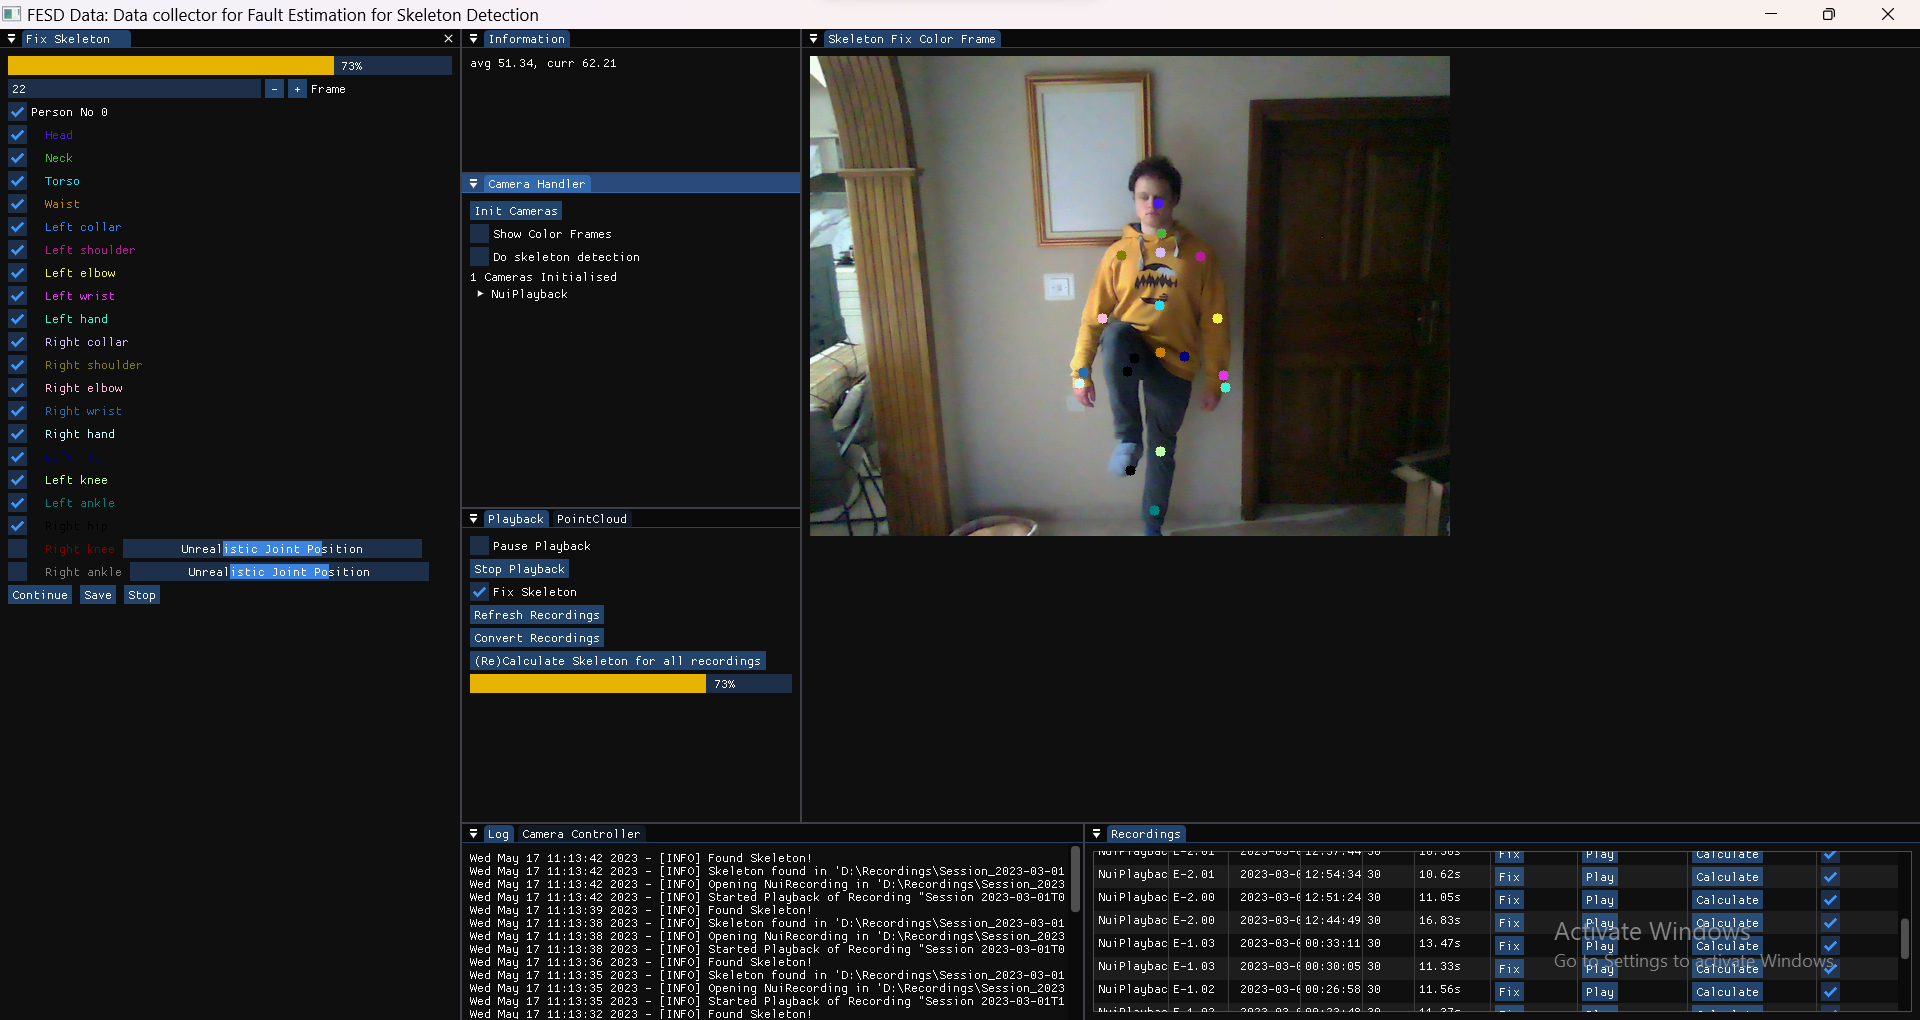
\includegraphics[width=\textwidth]{figures/FESDData/labelling.png}
  \end{subfigure}
  \caption[FESDData user interface]{A screenshot of the user interface with its two main components. On the left side, the user interface during streaming and recording can be seen and on the right side an example of data labelling.}
  \label{fig:fesddata}
\end{figure}  
